\chapter{Energy Loss Calculation}
Energy loss calculation for beam and charged fragment particles is performed using FORTRAN code: \textsc{elos} \cite{elos}. \textsc{elos} is a computer program which calculates time propagation of a charged particle in matter. In this code, the stopping power formula extracted from \textsc{rangelbl} \cite{rangelbl} are used. The material information between F7 to target and from target to SAMURAI entrance is recalculated from reference \cite{Dayonewiki} \cite{Ogoshi}

\section{Material Between F7 to Target}
\begin{table}[h]
    \centering
    \begin{tabular}{lcccc}
        \hline
    Detector & Composition & Phase  & Density  \\
    \hline
    Vacuum   & Vacuum & Gas &   \\
    Air      & N$_2$ :78\%, O$_2$ :21\%, Ar:1\% & Gas & 1.205 (mg/cm$^3$) \\
    Myler    & C$_{10}$H$_8$O$_4$ & Solid   & 1.400 (g/cm$^3$)\\
    Kapton   & C$_{22}$H$_{10}$N$_2$O$_5$ & Solid   & 1.420 (g/cm$^3$) \\
    Plastic  & C$_2$H$_4$ & Solid &  1.032 (g/cm$^3$) \\
    Vinylchloride & C$_2$H$_3$Cl & Solid &  1.300 (g/cm$^3$) \\
    Ar       & Ar      & Gas  & 1.662 (mg/cm$^3$) \\
    CH$_4$   & CH$_4$  & Gas  & 0.667 (mg/cm$^3$) \\
    C$_4$H$_{10}$ & C$_4$H$_{10}$ & Gas & 2.493 (mg/cm$^3$) \\
    \hline
    \end{tabular}
    \caption{Material information between F7 to target}
\end{table}

\begin{table}[h]
    \centering
    \begin{tabular}{lllll} \\ \hline
    \# & Detector   &Material Data & Thickness   & Note\\
       & or Vacuum  &      & (cm)        & \\
    \hline
    %s\multicolumn{5}{c}{F7} & 0.0 &  & \\ \hline
    1 & Vacuum      & vacuum.dat  &  11.041 &   11.0455+0.0045=11.05 \\
    2 & F7 PPAC 1   & mylar.dat   &  0.0045 &\\
    3 & F7 PPAC 2   & mylar.dat   &  0.0045 &\\ \hline
    4 & Vacuum      & vacuum.dat  &  9.3    &9.3+0.3+1.4=11.0 \\
    5 & Vacuum      & vacuum.dat  &  0.3    &\\
    6 & F7 Plastic  & plastic.dat &  1.4    &\\ \hline
    7 & Vacuum      & vacuum.dat  &  3576.35&3576.35+69.3=3645.65 \\
    \cline{1-4}
    8 & Vacuum      & vacuum.dat  & 69.3    & \\\hline
    9 & Kapton      & kapton.dat  & 0.0125  & 0.0125+11.9875=12.0 \\
    10& Air         & air.dat     & 11.9875 & \\\hline
    11& SBT1 Plastic& plastic.dat & 0.05    &0.05+0.02+0.0048  \\
    12& Light Shield&vinylchloride.dat& 0.02&+7.9252=8.0     \\
    13& Light Shield&  mylar.dat  & 0.0048  & \\
    \cline{1-4}
    14 & Air     & air.dat     & 7.9252  &   \\ 
    \hline
    15& SBT2 Plastic& plastic.dat & 0.05    & 0.05+0.02+0.0048\\
    16& Light Shield& vinylchloride.dat& 0.02& +5.9252=6.0\\
    17& Light Shield& mylar.dat  & 0.0048 & \\
    \cline{1-4}
    18 & Air     & air.dat    & 5.9252 &  \\\hline
    19 & ICB(Window)& kapton.dat & 0.003  & 0.003+22.98096 \\
    20 & ICB(Ar)    & Ar.dat     &22.98096& +2.55344+0.0126\\
    21 & ICB(CH$_4$)& CH4.dat    &2.55344 & +0.0126+2.55344 \\
    22 & ICB(Anode) & mylar.dat  & 0.0126 & +22.98096+0.003=51.1 \\
    23& ICB(Cathode)& mylar.dat  & 0.0126 &  \\
    24 & ICB(CH$_4$)& CH4.dat    &2.55344 &  \\
    25 & ICB(Ar)    & Ar.dat     &22.98096&  \\
    26 & ICB(Window)& kapton.dat & 0.003  & \\
    \hline
    27 & Air        & air.dat    & 5.0    & \\
    \hline
    28 &Window      & kapton.dat & 0.008  &0.008+14.079=14.087 \\
    29 &Vacuum      & vacuum.dat & 14.079  & \\
    \hline
    \end{tabular}
\end{table}

\begin{table}[h]
    \centering
    \begin{tabular}{lllll} \\ \hline
        \# & Detector   & Material Data & Thickness & Note    \\
           & or Vacuum  &                & (cm)      & \\
        \hline
    30 & BDC1(Window) & kapton.dat & 0.008 & 0.008+8.976 \\
    31 & BDC1(C$_4$H$_{10}$ 100 torr) & C4H10\_100torr.dat & 8.976 &    +0.008+0.008=9.0  \\
    32 & BDC1(Cathode) & kapton.dat & 0.008 &    \\
    33 & BDC1(Window)& kapton.dat & 0.008 &\\
    \hline
    34 & Vacuum     & vacuum.dat &90.932  &\\
    \hline
    35 & BDC2(Window) & kapton.dat & 0.008 &
    0.008+8.976 \\
    36 & BDC2(C$_4$H$_{10}$ 100 torr) & C4H10\_100torr.dat & 8.976 &    +0.008+0.008=9.0 \\
    37 & BDC2(Cathode)& kapton.dat & 0.008  &    \\
    38 & BDC2(Window) & kapton.dat & 0.008 & \\
    \hline
    39 & Vacuum    & vacuum.dat &97.281 & \\
    \hline
    40-1 & C Target(1/2 Thickness)& carbon\_1789.dat & 0.5  & Density: 1.789 g/cm$^3$ \\ 
    40-2 & Pb Target(1/2 Thickness)& Pb.dat & 0.1435  & Density: 11.34 g/cm$^3$ \\ \hline
    \end{tabular}
    \caption{List of material between F7 to target}
\end{table}

\begin{table}[h]
    \centering
    \begin{tabular}{lllll} \\ \hline
    \# & Detector   & Material Data & Thickness & Note    \\
       & or Vacuum  &         & (cm)     & \\
    \hline
    1-1 & C Target(1/2 Thickness) & carbon\_1789.dat & 0.5 & Density: 1.789 g/cm$^3$  \\ 
    1-2 & Pb Target(1/2 Thickness) & Pb.dat & 0.1435 & Density: 11.34 g/cm$^3$  \\ \hline
    2 & Vacuum      & vacuum.dat  & 97.338   \\ \hline
    3 & FDC1(Window) & kapton.dat & 0.016   & 0.016+0.012 \\
    4 & FDC1(Cathode)   & kapton.dat & 0.012   & +33.572=33.6\\
    5 & FDC1(C$_4$H$_{10}$ 50 torr) & C4H10\_50torr.dat & 33.572 &  \\
    \hline
    \end{tabular}
    \caption{List of material between target to FDC1}
\end{table}

\clearpage

\section{Energy Loss Calculation for Secondary Beam Particle}
For the evaluation of the secondary beam energy at the middle of target, energy loss calculation from F7 to the middle of target have performed. The initial energy is obtained from the $A/Z$ and the $B\rho$ at F5. After F5 to the middle of target, the energy loss calculation is performed using the \textsc{elos} code with the material information between F7 to target. The initial energy at F5 is given by the formula from \cite{Defour} as,
\begin{align}
E_{\text{F5}} = m_u \bigg( \sqrt{1+96.52\frac{B\rho^2}{m_u (A/Z)^2}} -1 \bigg),
\end{align}
where $m_u$ is the atomic mass unit, $B\rho$ is the magnetic rigidity from eq. \ref{eq:brho}, $A/Z$ from eq. \ref{eq:az}. The \textsc{eloss} calculation result is shown in Fig.\ref{fig:elos}. After the \textsc{eloss} calculation, the $\beta_{\text{tgt}}$ is obtained by 2nd order polynomial fitting as a function of $\text{TOF}_{\text{F7-F13}}$ and $E_{\text{tgt}}$ is calculated from the $\beta_{\text{tgt}}$.
\begin{align}
    \beta_{\text{tgt}} &= p_0 \cdot \text{TOF}_{\text{F7}-\text{F13}}^2 + p_1 \cdot \text{TOF}_{\text{F7}-\text{F13}} + p_2 \\
    E_{\text{tgt}} &= \frac{m_u}{\sqrt{1-\beta_{\text{tgt}}^2}}
 \end{align}
where $p_0$, $p_1$ and $p_2$ are the fitting parameters.

\begin{figure}[h]
    \centering
    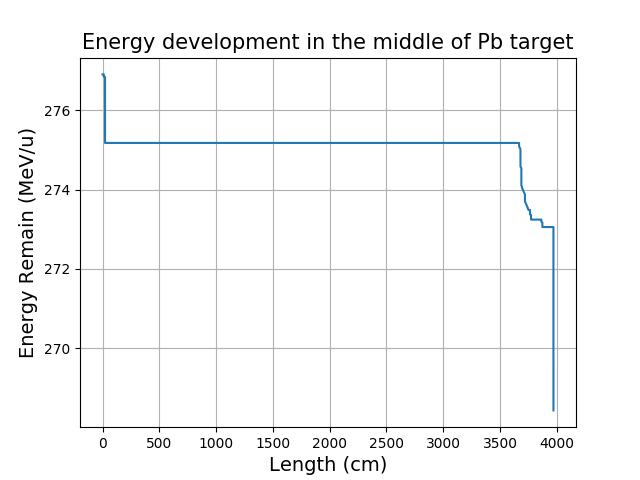
\includegraphics[width=0.6\textwidth]{energy.png}
    \caption{Energy development for $^{17}$B particle ($E_{\text{F5}} =$ 276.9 MeV/u) between F7 to Pb target}
    \label{fig:elos}
\end{figure}


\section{Momentum Push-back Calculation for Charged Fragment Particle}
We obtained the momentum of charged fragment particle in the vacuum of SAMURAI magnet by Geant4 simulation. For the invariant mass calculation, the momentum in the vacuum of SAMURAI magnet should be converted to the momentum in the middle of target. The momentum push-back calculation is performed using the \textsc{elos} code with the consideration energy loss in the material between SAMURAI magnet and the middle of target. The fitting function for momentum push-back calculation is given by
\begin{align}
    &P_{\text{SAMURAI}} = B\rho \times Z \times m_u\\
    &P_{\text{tgt}} = p_0 \cdot P_{\text{SAMURAI}} + p_1
\end{align}
where $P$ and $B\rho$ is the momentum and magnetic rigidity calculated by \textsc{eloss} code, $Z$ is the charge of the particle, $m_u$ is the atomic mass unit. $P_{\text{tgt}}$ and $P_{\text{SAMURAI}}$ is the momentum in the middle of target and the momentum in the vacuum of SAMURAI magnet, respectively. $p_0$ and $p_1$ are the fitting parameters. The fitting parameters are obtained by the linear fitting of the momentum push-back calculation result. Figure \ref{fig:momentum_pushback} shows the leaner fitting result for the momentum push-back calculation of $^{15}$B fragment particle for the C, Pb and empty target.

\begin{figure}[h]
    \centering
    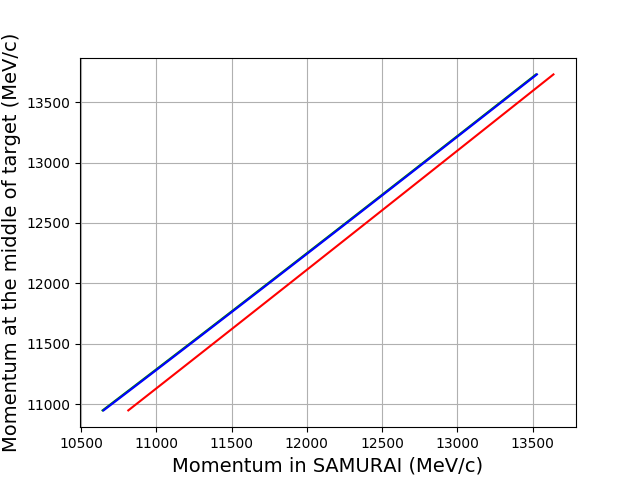
\includegraphics[width=0.6\textwidth]{momentum.png}
    \caption[Momentum push-back calculation for $^{15}$B fragment particle]{Momentum push-back calculation for $^{15}$B fragment particle. Blue line is for C and Pb target and red line is for empty target.}
    \label{fig:momentum_pushback}
\end{figure}